%% Loading packages
\usepackage{amsmath} % For cases in equations.
\usepackage{amsfonts} % For maths sets.
\usepackage{amssymb} % Square symbol for QED
\usepackage{physics} % For \abs{} and \norm{}.
\usepackage[inkscapelatex=false]{svg} %svg graphics
\usepackage{siunitx} % units formatting

\usepackage[backend=biber,style=numeric,citestyle=numeric-comp,maxcitenames=99,dateabbrev=false]{biblatex}
\addbibresource{biblio.bib}
\usepackage{setspace} % Bibliography spacings
\DeclareSourcemap{
  \maps[datatype=bibtex]{
    \map[overwrite]{
      \step[fieldsource=doi, final]
      \step[fieldset=url, null]
      \step[fieldset=eprint, null] }}}
\setcounter{biburllcpenalty}{7000} % break long url in bibliography
\setcounter{biburlucpenalty}{8000}
\renewcommand*{\bibfont}{\footnotesize} % bibliography font size
% Format of biblatex urldate in the bibliography.
\DeclareFieldFormat{urldate}{%
  Visited on \thefield{urlday}\addspace%
  \mkbibmonth{\thefield{urlmonth}}\addspace%
  \thefield{urlyear}\isdot}
\usepackage[ruled,vlined]{algorithm2e} % Algorithms.
\DontPrintSemicolon
\SetKwInOut{Input}{Input}\SetKwInOut{Output}{Output}
\usepackage{mathtools} % Ceiling function.
\usepackage{outlines} % Nest lists.
\usepackage{interval} % Writing intervals.
\usepackage[font={footnotesize,sf}]{caption} %Caption for figures in minipages.
\usepackage{floatrow}
% Figure captions always below. Figures always centered.
\floatsetup[figure]{capposition=bottom,objectset=centering}
\usepackage{wrapfig} %Wrapping figure with text.
\usepackage{stmaryrd} % Double brackets for integers interval.
\usepackage{doi} % Hyperlink DOI
\usepackage{etoolbox} %Ragged right bibliography.
\usepackage{color, colortbl} % Coloring rows in tables.
\usepackage{subcaption} % Subfigures.
\usepackage{pdfpages} % Include PDF pages.
\usepackage{epigraph} % Quotations at beginning of chapters.
\usepackage[en-GB]{datetime2} % Dates formatting
\DTMlangsetup{abbr,ord=omit,monthyearsep={\space}}
\setlength\epigraphwidth{.8\textwidth}
\usepackage[acronym,nonumberlist,nogroupskip,nopostdot]{glossaries} % Glossary for acronyms.
\renewcommand*{\glstextformat}[1]{\textcolor{black}{#1}} % No color on links for abbrev.

\DeclarePairedDelimiter{\ceil}{\lceil}{\rceil} % Ceiling function.
\DeclarePairedDelimiter{\floor}{\lfloor}{\rfloor} % Floor function.

\DeclareMathOperator*{\argmin}{argmin}

\setcounter{tocdepth}{3} % Table of content depth
\setcounter{secnumdepth}{3} % Section numbering depth

% Non-breaking around footnotes.
\makeatletter
\let\Footnote\footnote
\def\pst@@killglue{\unskip\ifdim\lastskip>\z@\expandafter\pst@@killglue\fi}
\def\footnote{\pst@@killglue\Footnote}
\makeatother

% More space below equations
\appto\normalsize{\belowdisplayshortskip=\belowdisplayskip}

% Rewrite month codes in bibliography
\DeclareSourcemap{
  \maps[datatype=bibtex]{
    \map[overwrite]{
      \step[fieldsource=month, match=\regexp{\A(j|J)an(uary)?\Z}, replace=1]
      \step[fieldsource=month, match=\regexp{\A(f|F)eb(ruary)?\Z}, replace=2]
      \step[fieldsource=month, match=\regexp{\A(m|M)ar(ch)?\Z}, replace=3]
      \step[fieldsource=month, match=\regexp{\A(a|A)pr(il)?\Z}, replace=4]
      \step[fieldsource=month, match=\regexp{\A(m|M)ay\Z}, replace=5]
      \step[fieldsource=month, match=\regexp{\A(j|J)un(e)?\Z}, replace=6]
      \step[fieldsource=month, match=\regexp{\A(j|J)ul(y)?\Z}, replace=7]
      \step[fieldsource=month, match=\regexp{\A(a|A)ug(ust)?\Z}, replace=8]
      \step[fieldsource=month, match=\regexp{\A(s|S)ep(tember)?\Z}, replace=9]
      \step[fieldsource=month, match=\regexp{\A(o|O)ct(ober)?\Z}, replace=10]
      \step[fieldsource=month, match=\regexp{\A(n|N)ov(ember)?\Z}, replace=11]
      \step[fieldsource=month, match=\regexp{\A(d|D)ec(ember)?\Z}, replace=12]}}}

% Footnotes marker color
\renewcommand\thefootnote{\textcolor{blue}{\arabic{footnote}}}

\pdfsuppresswarningpagegroup=1 % Silence warnings about pagegroups for figures.
\pdfminorversion=6 % PDF version 1.6 since we include articles in 1.6.

% Allow an extra pass to fix overfull hboxes by allowing more whitespace.
\emergencystretch=1em

% Page numbering and copyright notice.
\usepackage{fancyhdr}
\usepackage{lastpage}

\fancypagestyle{FirstPage}{
\fancyhf{} % Clear footer.
\rfoot{\thepage \hspace{1pt} of \pageref*{LastPage}}
\renewcommand{\headrulewidth}{0pt} % Remove rule at top of page
\lfoot{\href{https://creativecommons.org/licenses/by/4.0/}
       {\includesvg[inkscapelatex=false,height=14pt]{images/ccby.svg}}}
\lhead{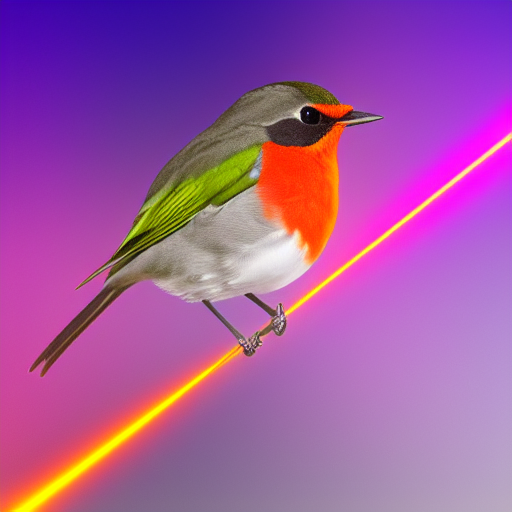
\includegraphics[height=64pt]{images/robintrace-logo.png}}
\chead{RobinTrace}
}

\fancypagestyle{plain}{
\fancyhf{} % Clear footer.
\rfoot{\thepage \hspace{1pt} of \pageref*{LastPage}}
\renewcommand{\headrulewidth}{0pt} % Remove rule at top of page
}

% Version history
\usepackage{vhistory}

% Keywords
\providecommand{\keywords}[1]{\textbf{Keywords --} #1}

% Glossary
\makeglossaries
\loadglsentries{glossary/glossary.tex}

\usepackage{fontawesome} %inline icons
\usepackage{xcolor}
\usepackage{listings} % Code listings
\definecolor{codeback}{rgb}{0.99,0.99,0.98}
\definecolor{codecomment}{HTML}{0588fc}
\definecolor{codekeyword}{HTML}{af5f00}
\definecolor{codestring}{HTML}{ffa07a}
\lstdefinestyle{mystyle}{
  backgroundcolor=\color{codeback},
  commentstyle=\color{codecomment},
  keywordstyle=\color{codekeyword},
  stringstyle=\color{codestring},
  basicstyle=\ttfamily\footnotesize,
  breakatwhitespace=false,         
  breaklines=true,                 
  captionpos=b,                    
  keepspaces=true,                 
  numbers=left,                    
  numbersep=5pt,                  
  showspaces=false,                
  showstringspaces=false,
  showtabs=false,                  
  tabsize=2}
\lstset{style=mystyle}

\usepackage[capitalise,nameinlink]{cleveref} % Include eg. "Fig." in front of figures.
\crefname{algorithm}{Alg.}{Algs.}
\crefname{table}{Tab.}{Tabs.}
\crefname{equation}{Eq}{Eqs.}
% Equation cross-references.
%\creflabelformat{equation}{#2#1#3}
\crefformat{equation}{(#2Eq.\thinspace#1#3)}

% No parentheses in equation labels.
%\newtagform{noparen}{}{}
%\usetagform{noparen}

